% ============================================================
% Capítulo 01: Modelagem de Negócio e Arquitetura com RM-ODP
% ============================================================
\chapter{Modelagem de Negócio e Arquitetura com RM-ODP}

\section{Introdução}

Antes de escrever uma única linha de código, o engenheiro de software precisa
responder a duas perguntas fundamentais: \textbf{o que} estamos construindo e
\textbf{por quê}. Essas perguntas podem parecer triviais, mas a realidade da
indústria mostra que a maioria dos fracassos em projetos de software não decorre
de falhas técnicas --- decorre de \textbf{falhas de entendimento}. O sistema foi
construído corretamente, mas era o sistema errado. Ou pior: ninguém concordava
sobre qual era o sistema certo.

A lacuna entre os requisitos de negócio e a implementação técnica é um abismo
silencioso. Ela não aparece nos sprints, não gera alertas no Jira e raramente é
discutida nas retrospectivas. Mas é precisamente nesse vácuo que moram os maiores
desastres: sistemas que custaram milhões e nunca foram usados, migrações que
paralisaram empresas, arquiteturas que pareciam elegantes no quadro branco mas
colapsaram sob carga real.

Dois frameworks conceituais nos oferecem uma estrutura disciplinada para atravessar
esse abismo. O primeiro é o \textbf{IDEF-0} (Integration DEFinition for Function
Modeling), que nos permite modelar processos de negócio de forma sistemática,
decompondo funções complexas em subfunções progressivamente mais detalhadas. O
segundo é o \textbf{RM-ODP} (Reference Model for Open Distributed Processing),
um padrão ISO que organiza o pensamento arquitetural em cinco vistas
complementares, cobrindo desde a motivação de negócio até as escolhas tecnológicas
concretas.

\begin{quote}
\textit{``A arquitetura de um sistema é determinada mais pelas suas restrições do que pelas suas funcionalidades.''} --- Adaptado de Fred Brooks
\end{quote}

Juntos, IDEF-0 e RM-ODP formam uma \textbf{espinha dorsal de pensamento} que
impede o engenheiro de cometer o erro mais comum e mais caro: pular direto para a
solução. O IDEF-0 conecta o negócio à funcionalidade; o RM-ODP conecta a
funcionalidade à arquitetura. Quando combinados com práticas como Spec Driven
Development e TDD, eles criam um pipeline intelectual que vai da compreensão do
problema até a validação da solução, sem atalhos perigosos.

Na era da inteligência artificial generativa, esses modelos são ainda mais
valiosos. Um LLM pode gerar código em segundos, mas ele não sabe \emph{qual}
código gerar sem contexto adequado. IDEF-0 e RM-ODP fornecem exatamente isso:
\textbf{contexto estruturado} para os prompts e \textbf{critérios objetivos}
para validar o código gerado. Como discutimos no Capítulo~0, o diferencial do
engenheiro não é escrever código --- é \emph{saber qual código escrever}. Este
capítulo lhe dará as ferramentas para fazer isso com rigor.

Ao longo das próximas seções, vamos construir um exemplo completo: modelaremos
um \textbf{sistema de e-commerce} desde o nível mais abstrato do negócio até as
escolhas tecnológicas concretas, passando por todas as cinco vistas do RM-ODP.
Você verá como cada vista ilumina um aspecto diferente do problema e como, juntas,
elas eliminam as ambiguidades que costumam assombrar projetos reais.


% ============================================================
\section{IDEF-0: Modelagem do Negócio}
% ============================================================

O IDEF-0 (Integration DEFinition for Function Modeling) nasceu em um contexto
bastante distante do software moderno. Foi criado na década de 1970 pela Força
Aérea dos Estados Unidos como parte do programa ICAM (Integrated Computer-Aided
Manufacturing), com o objetivo de modelar processos de manufatura de forma
rigorosa e padronizada. A necessidade era clara: sistemas de fabricação aeronáutica
são complexos demais para serem descritos informalmente, e qualquer ambiguidade
poderia ter consequências catastróficas.

O que torna o IDEF-0 relevante décadas depois, em um contexto de microsserviços e
inteligência artificial, é sua simplicidade conceitual aliada a um rigor
surpreendente. Ele nos obriga a pensar em processos usando um vocabulário
estruturado --- o acrônimo \textbf{ICOM} --- que elimina ambiguidades antes que
elas contaminem o design do sistema.

\subsection{O Paradigma ICOM}

Todo processo no IDEF-0 é definido por exatamente quatro tipos de elementos, dispostos
em posições fixas ao redor de uma caixa funcional:

\begin{description}[style=nextline]
    \item[\textbf{I}nputs (à esquerda)] O que entra no processo para ser
    transformado. São os dados, materiais ou informações que o processo consome.
    Em software, inputs típicos são requisições de usuários, dados de sensores,
    eventos de outros sistemas.

    \item[\textbf{C}ontrols (acima)] O que governa o processo sem ser consumido
    por ele. Regras de negócio, políticas organizacionais, legislação, padrões
    técnicos, SLAs. Controls são as \emph{restrições} sob as quais o processo
    opera. Um pedido de compra (input) é processado de acordo com a política
    de preços (control).

    \item[\textbf{O}utputs (à direita)] O que sai do processo como resultado
    da transformação. Produtos, serviços, decisões, notificações, dados
    transformados. A distinção é que outputs são o \emph{propósito} do processo
    --- a razão pela qual ele existe.

    \item[\textbf{M}echanisms (abaixo)] Quem ou o que executa o processo.
    Pessoas, sistemas, máquinas, APIs externas. Mechanisms são os
    \emph{viabilizadores} --- sem eles, o processo é apenas uma abstração.
\end{description}

A beleza do ICOM está na disciplina que ele impõe. Quando você se obriga a
classificar cada elemento como Input, Control, Output ou Mechanism, descobre
rapidamente onde seu entendimento é vago. ``O preço do produto é um input ou um
control?'' Se o preço é calculado pelo sistema, é um output de outro processo.
Se vem de uma tabela fixa, é um control. Se vem do fornecedor, é um input. Essa
distinção, que parece acadêmica, tem implicações diretas na arquitetura: inputs
precisam de interfaces de entrada, controls precisam de repositórios de regras,
outputs precisam de canais de distribuição.

\subsection{Do Diagrama A-0 à Decomposição}

O IDEF-0 começa com o \textbf{diagrama A-0}: uma única caixa representando todo o
sistema em seu contexto mais amplo. Esse diagrama de contexto é deliberadamente
simplificado --- ele mostra \emph{o que} o sistema faz, não \emph{como}. É o
equivalente a descrever uma fábrica inteira como ``transforma matéria-prima em
produtos acabados''.

\begin{figure}[htbp]
    \centering
    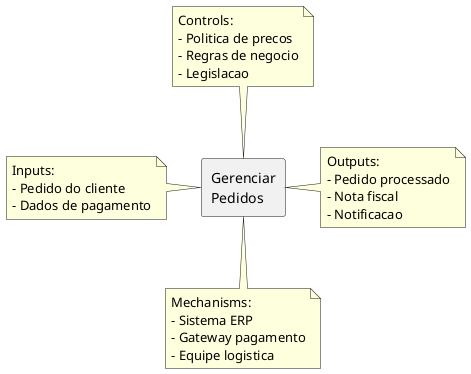
\includegraphics[width=0.85\textwidth]{imagens/01-modelagem-negocio-rm-odp-01-diagrama-idef-0-nivel-0-sistema-de-pedidos.png}
    \caption{Diagrama IDEF-0 Nível 0 -- Sistema de Pedidos}
\end{figure}

A partir do A-0, cada caixa pode ser \textbf{decomposta} em subfunções. Essa
decomposição segue uma regra prática importante: cada nível deve conter entre
3 e 6 subfunções. Menos de 3 sugere que o nível é desnecessário; mais de 6
indica que as funções precisam ser agrupadas em abstrações mais altas. Cada nível
responde à pergunta ``\emph{como?}'' em relação ao nível anterior.

\subsection{Exemplo Completo: Decomposição em Três Níveis}

Vamos decompor o sistema de pedidos do nosso e-commerce em três níveis
progressivos. Esse exercício ilustra como o IDEF-0 nos leva do abstrato ao
concreto sem perder o fio da meada.

\begin{figure}[htbp]
    \centering
    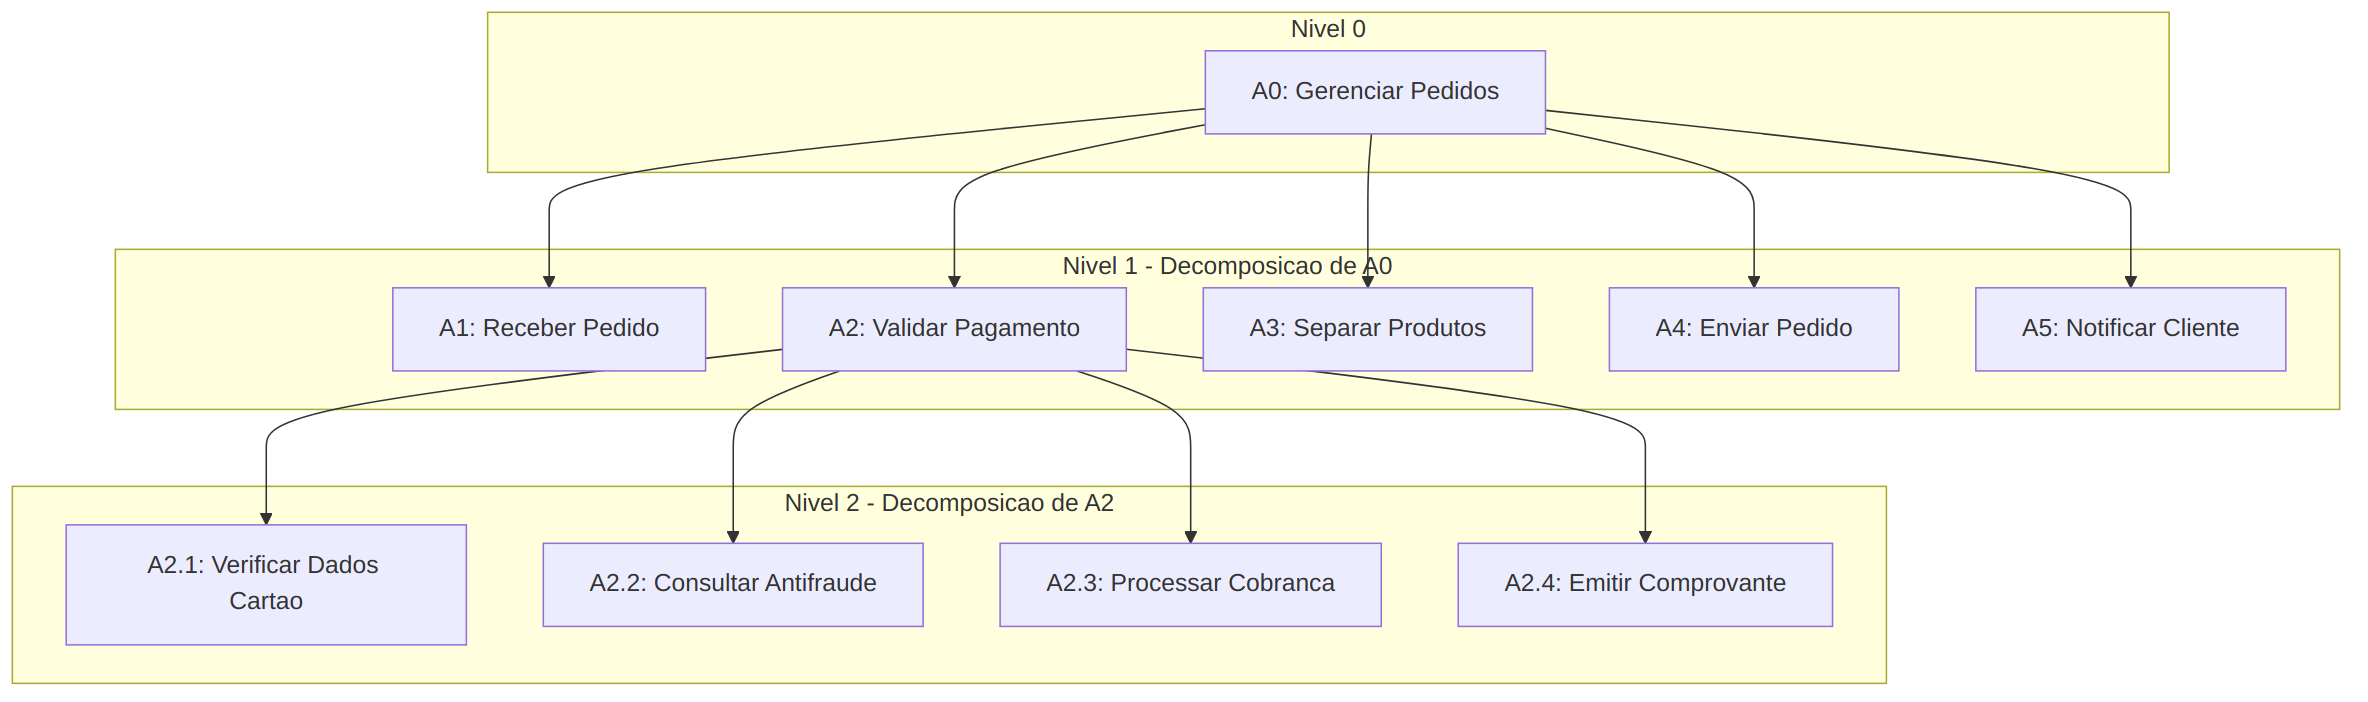
\includegraphics[width=0.85\textwidth]{imagens/01-modelagem-negocio-rm-odp-02-decomposicao-funcional-idef-0-em-3-niveis.png}
    \caption{Decomposicao Funcional IDEF-0 em 3 Niveis}
\end{figure}

\textbf{Nível 0} --- \emph{Gerenciar Pedidos}: a função raiz que representa todo
o escopo do sistema. Os inputs são o pedido do cliente e seus dados de pagamento.
Os controls incluem a política de preços, a legislação consumerista (CDC, LGPD)
e as regras de negócio da empresa. Os outputs são o pedido processado, a nota
fiscal eletrônica e as notificações ao cliente. Os mechanisms são o sistema ERP,
o gateway de pagamento e a equipe de logística.

\textbf{Nível 1} --- \emph{Decomposição de A0}: o processo de gerenciar pedidos
se decompõe em cinco subfunções. ``Receber Pedido'' (A1) captura e valida os dados
iniciais. ``Validar Pagamento'' (A2) processa a transação financeira. ``Separar
Produtos'' (A3) orquestra o processo de \emph{picking} no estoque. ``Enviar
Pedido'' (A4) gerencia a logística de entrega. ``Notificar Cliente'' (A5)
mantém o cliente informado ao longo de todo o ciclo.

\textbf{Nível 2} --- \emph{Decomposição de A2 (Validar Pagamento)}: a função de
validação de pagamento, por sua complexidade e criticidade, merece uma decomposição
adicional. ``Verificar Dados do Cartão'' (A2.1) valida formato, data de validade e
bandeira. ``Consultar Antifraude'' (A2.2) envia os dados para um serviço de análise
de risco. ``Processar Cobrança'' (A2.3) efetua a transação junto à adquirente.
``Emitir Comprovante'' (A2.4) gera o registro da transação para o cliente e para
o sistema contábil.

Observe como o \textbf{node index} --- a numeração A0, A1, A2.1 --- permite
rastrear a origem de cada função. Quando alguém pergunta ``de onde veio esse
microsserviço de antifraude?'', a resposta é clara: é a realização técnica de
A2.2, que faz parte de A2 (Validar Pagamento), que faz parte de A0 (Gerenciar
Pedidos). Essa rastreabilidade é ouro em projetos complexos.

\subsection{IDEF-0 na Era da IA}

Os LLMs atuais são capazes de gerar diagramas IDEF-0 a partir de descrições
textuais, e essa capacidade é genuinamente útil para acelerar a fase inicial de
modelagem. No entanto, \textbf{validar o modelo} continua sendo responsabilidade
exclusiva do engenheiro. Um LLM não sabe se sua empresa tem uma política de
devolução em 7 dias ou em 30 dias. Ele não sabe que o serviço de antifraude é
um requisito regulatório no seu segmento. Ele vai gerar algo plausível, mas
``plausível'' não é o mesmo que ``correto''.

A abordagem recomendada é usar a IA como \emph{rascunhadora}: peça a ela para
gerar uma primeira versão do IDEF-0, depois revise criteriosamente cada elemento
ICOM. Pergunte-se: ``Esse input realmente existe? Esse control está documentado?
Esse mechanism está disponível? Esse output é o que o stakeholder espera?''


% ============================================================
\section{RM-ODP: Reference Model for Open Distributed Processing}
% ============================================================

Se o IDEF-0 nos ajuda a entender \emph{o negócio}, o RM-ODP nos ajuda a pensar
\emph{a arquitetura}. O RM-ODP (ISO/IEC 10746) é um padrão internacional que
organiza a especificação de sistemas distribuídos em \textbf{cinco vistas}
(viewpoints) complementares. Cada vista é uma lente diferente sobre o mesmo
sistema, respondendo um tipo específico de pergunta.

É importante entender o que o RM-ODP \emph{não} é. Ele não é um framework
prescritivo que dita como construir sistemas. Não é uma metodologia com fases
sequenciais. Não é um conjunto de templates a serem preenchidos mecanicamente.
O RM-ODP é, fundamentalmente, uma \textbf{lente de pensamento} --- uma forma
disciplinada de garantir que você considerou todos os aspectos relevantes de
um sistema antes de construí-lo.

\begin{quote}
\textit{``Cada vista do RM-ODP ilumina um aspecto do sistema que as outras deixam
no escuro. Ignorar uma vista é como projetar um edifício sem considerar a
fundação --- pode parecer completo, mas não vai se sustentar.''}
\end{quote}

A analogia mais útil é a da planta de um edifício. Um arquiteto civil não
trabalha com uma única planta; ele cria plantas elétricas, hidráulicas,
estruturais, de acabamento e de paisagismo. Cada planta mostra o mesmo
edifício sob uma perspectiva diferente, e é a \emph{consistência} entre elas
que garante que o prédio funcionará. O RM-ODP faz o mesmo para sistemas de
software: são cinco ``plantas'' que, juntas, cobrem do ``por quê'' ao ``com
quê''.

\begin{figure}[htbp]
    \centering
    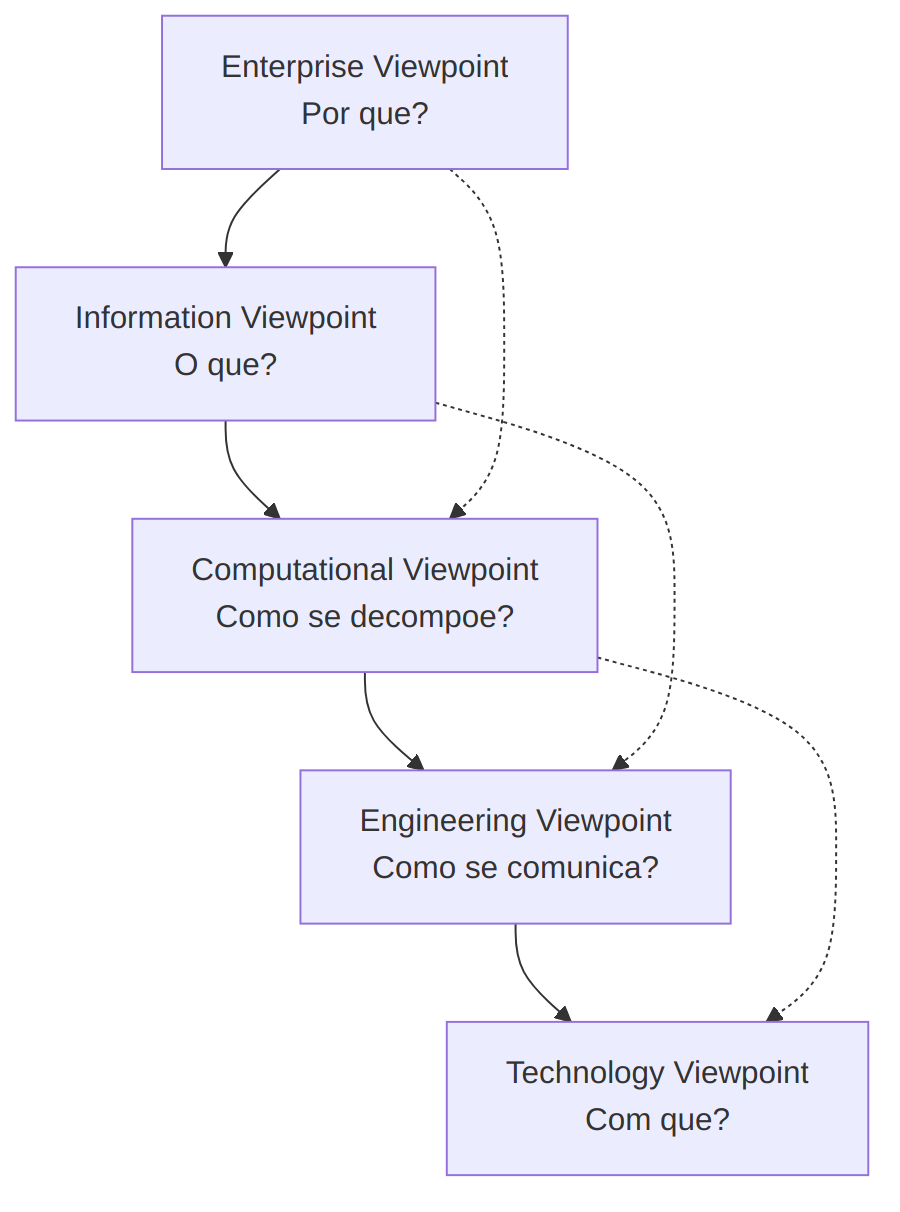
\includegraphics[width=0.85\textwidth]{imagens/01-modelagem-negocio-rm-odp-03-as-cinco-vistas-do-rm-odp-e-suas-relacoes.png}
    \caption{As Cinco Vistas do RM-ODP e suas Relacoes}
\end{figure}

Originalmente concebido para sistemas distribuídos na década de 1990, o RM-ODP
se aplica com perfeição a \textbf{qualquer} sistema de software moderno ---
especialmente em um mundo onde praticamente todo sistema é, de alguma forma,
distribuído. Mesmo uma aplicação aparentemente monolítica que usa um banco de
dados externo, um serviço de e-mail e uma CDN já é, na prática, um sistema
distribuído.

Nas próximas subseções, exploraremos cada uma das cinco vistas usando nosso
exemplo de e-commerce como fio condutor.

\subsection{Enterprise Viewpoint --- A Vista Empresarial}

A Enterprise Viewpoint é a vista que responde à pergunta mais fundamental:
\textbf{por que este sistema existe?} Ela lida com o contexto organizacional,
os objetivos de negócio, os stakeholders e as políticas que governam o sistema.
É a vista que conecta a tecnologia ao propósito.

Muitos engenheiros de software consideram essa vista ``trabalho do analista de
negócios'' e a ignoram. Esse é um erro caro. Sem uma compreensão clara do
propósito empresarial, decisões arquiteturais são tomadas no vácuo. Você pode
projetar um sistema com 99,999\% de disponibilidade quando o negócio toleraria
99,9\% --- gastando dez vezes mais sem necessidade. Ou, inversamente, projetar
para 99\% quando o negócio exige 99,99\% --- criando uma bomba-relógio.

Para o nosso e-commerce, a Enterprise Viewpoint nos revela:

\begin{description}[style=nextline]
    \item[Propósito] Permitir que clientes comprem produtos online com entrega
    rápida e confiável, gerando receita sustentável para a empresa.

    \item[Stakeholders] Clientes finais (compram produtos), vendedores/lojistas
    (ofertam produtos), equipe de logística (entrega), equipe financeira
    (conciliação e relatórios), equipe jurídica (conformidade regulatória),
    time de tecnologia (manutenção e evolução).

    \item[Políticas e regulamentações] Lei Geral de Proteção de Dados (LGPD),
    Código de Defesa do Consumidor (CDC), política interna de devolução em
    até 7 dias, política de preços com markup mínimo de 15\%.

    \item[Requisitos de qualidade (SLAs)] Disponibilidade de 99,9\% (máximo
    de 8,76 horas de indisponibilidade por ano), tempo de resposta do checkout
    inferior a 3 segundos no percentil 95, recuperação de desastres em até
    4 horas (RTO), perda máxima de dados de 1 hora (RPO).

    \item[Métricas de sucesso] Taxa de conversão do carrinho acima de 3\%,
    NPS acima de 50, tempo médio de entrega inferior a 48 horas, taxa de
    devolução abaixo de 5\%.
\end{description}

A \textbf{conexão com o IDEF-0} é direta: os Controls e Mechanisms do diagrama
de nível mais alto \emph{são} a Enterprise Viewpoint. As políticas de preço,
a legislação e as regras de negócio que aparecem como Controls no IDEF-0 são
exatamente as políticas da Enterprise Viewpoint. O sistema ERP e o gateway de
pagamento que aparecem como Mechanisms são os viabilizadores que a Enterprise
Viewpoint identifica como recursos necessários.

\subsection{Information Viewpoint --- A Vista de Informação}

A Information Viewpoint responde à pergunta: \textbf{o que o sistema precisa
saber?} Ela se concentra na semântica da informação, independentemente de como
essa informação será processada ou armazenada. É a vista que define as entidades
do domínio, seus relacionamentos, suas regras de integridade e seus ciclos de vida.

Se a Enterprise Viewpoint é o ``porquê'', a Information Viewpoint é o ``o quê''.
Ela é deliberadamente agnóstica em relação à tecnologia: não importa se os dados
serão armazenados em PostgreSQL, MongoDB ou em rolos de papiro --- o que importa
é a \emph{estrutura semântica} da informação.

Para nosso e-commerce, as entidades centrais e seus relacionamentos são:

\begin{description}[style=nextline]
    \item[Cliente] Possui nome, CPF (único), e-mail (único), endereços de
    entrega (lista), histórico de pedidos. Um Cliente pode ter muitos Pedidos.

    \item[Produto] Possui SKU (único), nome, descrição, preço base, categoria,
    quantidade em estoque. Um Produto pode aparecer em muitos Itens de Pedido.

    \item[Pedido] Possui identificador único, referência ao Cliente, lista de
    Itens, valor total, status, timestamps de criação e atualização. Um Pedido
    pertence a um único Cliente e contém múltiplos Itens.

    \item[Item de Pedido] Representa a associação entre Pedido e Produto, com
    quantidade e preço unitário no momento da compra (snapshot).

    \item[Pagamento] Vinculado a um Pedido, contém método (cartão, PIX, boleto),
    status, valor, referência da transação no gateway.

    \item[Entrega] Vinculada a um Pedido, contém endereço de destino, código de
    rastreamento, transportadora, status, datas estimada e real de entrega.
\end{description}

As \textbf{invariantes} --- regras que devem ser verdadeiras em qualquer momento
--- são cruciais e frequentemente negligenciadas:

\begin{itemize}
    \item Um pedido não pode ter valor total negativo.
    \item A quantidade de itens em um pedido deve ser maior que zero.
    \item Um produto só pode ser adicionado a um pedido se houver estoque suficiente.
    \item O preço unitário de um item no pedido é congelado no momento da compra
    (não muda se o preço do produto mudar depois).
    \item Um pedido pago não pode ser alterado, apenas cancelado (com estorno).
    \item O CPF do cliente deve ser válido segundo o algoritmo de verificação.
\end{itemize}

O \textbf{ciclo de vida} da informação é outro aspecto fundamental. Um Pedido,
por exemplo, não nasce e permanece estático --- ele evolui ao longo do tempo
através de estados bem definidos:

\begin{center}
\texttt{Criado} $\to$ \texttt{Pagamento Pendente} $\to$ \texttt{Pago} $\to$
\texttt{Em Separação} $\to$ \texttt{Enviado} $\to$ \texttt{Entregue}
\end{center}

Com bifurcações possíveis para \texttt{Cancelado} (a partir de Criado ou
Pagamento Pendente) e \texttt{Devolvido} (a partir de Entregue). Cada transição
de estado tem pré-condições (o que precisa ser verdade para a transição ocorrer)
e pós-condições (o que deve ser verdade após a transição).

A \textbf{conexão com Domain-Driven Design} é natural e poderosa. As entidades
da Information Viewpoint correspondem diretamente às Entidades e Value Objects do
DDD. As invariantes correspondem às regras de negócio dos Agregados. As transições
de estado correspondem aos Domain Events. Se você já pratica DDD, a Information
Viewpoint vai parecer familiar --- e se não pratica, ela é uma excelente porta
de entrada, como exploraremos em mais detalhes no Capítulo~3.

\subsection{Computational Viewpoint --- A Vista Computacional}

A Computational Viewpoint responde à pergunta: \textbf{como o sistema se decompõe
em unidades funcionais?} Esta é a vista mais próxima do que os engenheiros
tradicionalmente chamam de ``arquitetura de software''. Ela define os objetos
computacionais (componentes), suas interfaces e as interações entre eles.

O aspecto mais importante --- e mais contraintuitivo --- desta vista é que ela é
\textbf{independente de distribuição e de tecnologia}. Na Computational Viewpoint,
não importa se dois componentes rodam no mesmo processo ou em continentes
diferentes. Não importa se se comunicam via HTTP, gRPC ou pombo-correio. O que
importa são as \emph{responsabilidades}, as \emph{interfaces} e os
\emph{contratos}.

Para nosso e-commerce, os objetos computacionais e suas interfaces são:

\begin{description}[style=nextline]
    \item[\texttt{CatalogoService}] Responsável pela gestão do catálogo de
    produtos. Interface: \texttt{buscarProduto(sku)},
    \texttt{listarProdutos(filtro, paginacao)},
    \texttt{atualizarEstoque(sku, quantidade)}.

    \item[\texttt{PedidoService}] Responsável pela criação e gestão do ciclo
    de vida dos pedidos. Interface: \texttt{criarPedido(cliente, itens)},
    \texttt{cancelarPedido(pedidoId)},
    \texttt{consultarPedido(pedidoId)},
    \texttt{atualizarStatus(pedidoId, novoStatus)}.

    \item[\texttt{PagamentoGateway}] Abstração sobre os provedores de pagamento.
    Interface: \texttt{processarPagamento(pedidoId, metodo, dados)},
    \texttt{consultarPagamento(transacaoId)},
    \texttt{estornarPagamento(transacaoId)}.

    \item[\texttt{EstoqueManager}] Responsável pela reserva e liberação de
    estoque. Interface: \texttt{reservarItens(itens)},
    \texttt{confirmarReserva(reservaId)},
    \texttt{liberarReserva(reservaId)},
    \texttt{consultarDisponibilidade(sku)}.

    \item[\texttt{NotificacaoDispatcher}] Responsável por enviar notificações
    ao cliente por múltiplos canais. Interface:
    \texttt{enviarNotificacao(destinatario, canal, template, dados)}.

    \item[\texttt{EntregaTracker}] Responsável pelo acompanhamento das entregas.
    Interface: \texttt{registrarEnvio(pedidoId, transportadora)},
    \texttt{consultarRastreamento(pedidoId)},
    \texttt{atualizarStatusEntrega(pedidoId, status)}.
\end{description}

As \textbf{interações} entre esses objetos podem ser síncronas (uma chamada que
espera resposta), assíncronas (uma mensagem que não espera resposta imediata) ou
baseadas em publicação/assinatura (um evento que múltiplos interessados podem
consumir). Na Computational Viewpoint, definimos a \emph{semântica} da interação,
não o \emph{mecanismo}:

\begin{itemize}
    \item \texttt{PedidoService} chama \texttt{EstoqueManager.reservarItens}
    sincronamente (precisa da confirmação antes de prosseguir).
    \item \texttt{PedidoService} publica o evento \texttt{PedidoCriado}, que
    \texttt{NotificacaoDispatcher} consome assincronamente.
    \item \texttt{PagamentoGateway} publica \texttt{PagamentoConfirmado}, que
    \texttt{PedidoService} e \texttt{EstoqueManager} consomem.
\end{itemize}

A conexão com padrões arquiteturais modernos é direta:

\begin{itemize}
    \item \textbf{Microsserviços}: cada objeto computacional pode se tornar um
    microsserviço independente.
    \item \textbf{Arquitetura Hexagonal}: cada objeto é um hexágono com portas
    de entrada (interfaces que oferece) e portas de saída (interfaces que consome).
    \item \textbf{Clean Architecture}: os objetos são organizados por camadas de
    abstração, com dependências apontando para dentro.
\end{itemize}

Exploraremos essas conexões com profundidade nos Capítulos~2 e~3.

\subsection{Engineering Viewpoint --- A Vista de Engenharia}

A Engineering Viewpoint responde à pergunta: \textbf{como os componentes se
comunicam e se distribuem na prática?} Se a Computational Viewpoint é o ``o
quê'' da arquitetura, a Engineering Viewpoint é o ``como na prática''. Ela trata
dos mecanismos de distribuição, dos protocolos de comunicação, das estratégias de
tolerância a falhas e dos requisitos de qualidade de serviço.

Esta é a vista onde a realidade do mundo distribuído se impõe com toda a sua
complexidade. Na Computational Viewpoint, dizer que ``PedidoService chama
EstoqueManager'' é suficiente. Na Engineering Viewpoint, precisamos especificar:

\begin{description}[style=nextline]
    \item[Protocolos de comunicação] \texttt{PedidoService} chama
    \texttt{EstoqueManager} via gRPC com TLS mútuo. Eventos são publicados
    via Apache Kafka com particionamento por \texttt{pedidoId}.

    \item[Qualidade de serviço] Chamadas síncronas têm timeout de 2 segundos.
    Mensagens assíncronas devem ser processadas em até 30 segundos. Throughput
    esperado: 500 pedidos por minuto no pico.

    \item[Tolerância a falhas] Retry com backoff exponencial (máximo 3 tentativas)
    para chamadas idempotentes. Circuit breaker com threshold de 50\% de falhas
    em janela de 30 segundos. Dead letter queue para mensagens que falharam
    após todas as tentativas. Fallback para cache local quando o serviço de
    catálogo está indisponível.

    \item[Consistência] Reserva de estoque usa o padrão Saga com compensação.
    Se o pagamento falha após a reserva, uma mensagem de compensação libera
    os itens reservados. Idempotência garantida por chave de idempotência
    no header.

    \item[Monitoramento] Distributed tracing com OpenTelemetry. Métricas de
    latência (p50, p95, p99) expostas via Prometheus. Logs estruturados em
    JSON com correlation ID.
\end{description}

A \textbf{conexão com DevOps} é profunda. Service meshes como Istio e Linkerd
implementam muitas das preocupações da Engineering Viewpoint de forma
transparente: retry, circuit breaking, mTLS, observabilidade. Message brokers
como Kafka e RabbitMQ implementam os padrões de comunicação assíncrona. API
gateways como Kong e AWS API Gateway implementam rate limiting, autenticação
e roteamento.

\subsection{Technology Viewpoint --- A Vista Tecnológica}

A Technology Viewpoint responde à pergunta final: \textbf{com quais tecnologias
concretas construímos?} Esta é a vista mais familiar para a maioria dos
engenheiros --- e, paradoxalmente, a que mais frequentemente é decidida
\emph{primeiro}, invertendo a ordem lógica. Escolher o banco de dados antes de
entender as invariantes da informação, ou escolher o framework antes de definir
as interfaces computacionais, é como escolher os tijolos antes de ter a planta
do edifício.

Para nosso e-commerce, as escolhas tecnológicas --- que só devem ser feitas
\emph{após} as quatro vistas anteriores --- poderiam ser:

\begin{description}[style=nextline]
    \item[Linguagens e frameworks] Python com FastAPI para
    \texttt{CatalogoService} e \texttt{PedidoService} (produtividade,
    ecossistema rico). Go para \texttt{PagamentoGateway} (performance,
    tipagem forte para domínio financeiro). TypeScript com NestJS para
    \texttt{NotificacaoDispatcher} (facilidade de integração com APIs de
    terceiros).

    \item[Bancos de dados] PostgreSQL para dados transacionais (pedidos,
    pagamentos) --- ACID, maturidade, suporte a JSON. Redis para cache de
    catálogo e sessões --- velocidade, TTL nativo. Elasticsearch para busca
    de produtos --- full-text search, faceted navigation.

    \item[Infraestrutura] Kubernetes (EKS) para orquestração de containers.
    Kafka (MSK) para eventos assíncronos. Terraform para
    Infrastructure-as-Code. Datadog para observabilidade.

    \item[Ferramentas de desenvolvimento] Docker para ambientes locais. GitHub
    Actions para CI/CD. SonarQube para análise estática. Swagger/OpenAPI para
    documentação de APIs.
\end{description}

A \textbf{conexão com ADRs} (Architecture Decision Records) é fundamental. Cada
decisão tecnológica significativa deve ser documentada como um ADR, registrando
o contexto, as alternativas consideradas, a decisão tomada e suas consequências.
``Por que PostgreSQL e não DynamoDB?'' --- o ADR explica que a consistência forte
era um requisito da Information Viewpoint e que o custo operacional do PostgreSQL
gerenciado (RDS) era aceitável para o volume esperado.


% ============================================================
\section{Estudo de Caso: E-commerce Atravessando as Cinco Vistas}
% ============================================================

Agora que exploramos cada vista individualmente, vamos consolidar o entendimento
percorrendo as cinco vistas de forma integrada para nosso sistema de e-commerce.
O objetivo é demonstrar como cada vista ilumina aspectos diferentes do mesmo
sistema e como a \textbf{consistência entre vistas} é tão importante quanto o
conteúdo de cada uma individualmente.

Imagine que você é o engenheiro líder de uma startup de e-commerce chamada
\emph{MarketBR}. A empresa vende produtos de diversos lojistas com entrega
própria. O CEO quer lançar a plataforma em 4 meses. Onde você começa?

\textbf{Passo 1 --- Enterprise Viewpoint}: você reúne os stakeholders (CEO,
head de logística, head financeiro, representante jurídico) e documenta: o
sistema deve permitir que clientes comprem de múltiplos lojistas em um único
carrinho, com pagamento unificado e entrega consolidada. O SLA de disponibilidade
é 99,9\%. O sistema deve estar em conformidade com LGPD e CDC. A meta é
processar 10.000 pedidos por dia no primeiro ano.

\textbf{Passo 2 --- Information Viewpoint}: com o propósito claro, você modela
as entidades. Descobre que ``Lojista'' é uma entidade que não existia no modelo
inicial. Descobre que ``Carrinho'' e ``Pedido'' são entidades distintas (o
carrinho é efêmero, o pedido é persistente). Descobre que o ``Valor Total''
precisa considerar frete por lojista. As invariantes revelam complexidades:
``um pedido multi-lojista gera múltiplos pagamentos ao fornecedor, mas um
único débito ao cliente''.

\textbf{Passo 3 --- Computational Viewpoint}: as entidades e invariantes guiam
a decomposição em componentes. O \texttt{CarrinhoService} é separado do
\texttt{PedidoService} porque têm ciclos de vida e requisitos de consistência
diferentes. O \texttt{SplitPaymentService} emerge como componente necessário
para gerenciar o split de pagamento entre lojistas. O \texttt{FreteCalculator}
precisa de interface com múltiplas transportadoras.

\textbf{Passo 4 --- Engineering Viewpoint}: a natureza multi-lojista impõe
requisitos específicos. O cálculo de frete deve ser paralelo (consultar
múltiplas transportadoras simultaneamente, com timeout agressivo de 1 segundo).
O split de pagamento é uma Saga com compensação --- se o débito ao cliente
falha, todas as reservas são liberadas. O catálogo de cada lojista é
eventualmente consistente com o catálogo central (replicado via eventos Kafka).

\textbf{Passo 5 --- Technology Viewpoint}: com todos os requisitos claros, as
escolhas tecnológicas se justificam. PostgreSQL para pedidos e pagamentos
(transações ACID). Redis para carrinho (efêmero, alta velocidade). Elasticsearch
para catálogo (busca full-text com filtros por lojista). Kafka para eventos
entre serviços. Kubernetes para orquestração. Stripe Connect para split de
pagamento.

Observe como cada passo depende dos anteriores. Sem a Enterprise Viewpoint, não
saberíamos que o split de pagamento era necessário. Sem a Information Viewpoint,
não teríamos descoberto a entidade Lojista. Sem a Computational Viewpoint, não
teríamos separado carrinho de pedido. Sem a Engineering Viewpoint, não teríamos
definido a estratégia de consistência. E sem tudo isso, as escolhas tecnológicas
seriam chutes educados, não decisões informadas.


% ============================================================
\section{Mapeando IDEF-0 e RM-ODP: A Matriz de Rastreabilidade}
% ============================================================

Um dos maiores valores de usar IDEF-0 e RM-ODP em conjunto é a capacidade de
criar uma \textbf{matriz de rastreabilidade} --- um mapeamento explícito entre
os elementos de cada framework. Essa matriz serve como detector de lacunas e
inconsistências: se uma função do IDEF-0 não aparece em nenhuma vista do RM-ODP,
algo foi esquecido. Se a Enterprise Viewpoint promete ``entrega em 48 horas'' mas
a Engineering Viewpoint usa processamento em lote diário, há uma contradição que
precisa ser resolvida antes que se torne um bug em produção.

\begin{table}[htbp]
\centering
\caption{Mapeamento entre Elementos IDEF-0 e Vistas RM-ODP}
\label{tab:idef-odp-mapping}
\begin{tabular}{@{}p{2.8cm}p{2.2cm}p{2.2cm}p{2.2cm}p{2.2cm}p{2.2cm}@{}}
\toprule
\textbf{Elemento IDEF-0} & \textbf{Enterprise} & \textbf{Information} &
\textbf{Computational} & \textbf{Engineering} & \textbf{Technology} \\
\midrule
\textbf{Inputs} & Necessidades dos stakeholders & Entidades e dados de entrada &
Parâmetros das interfaces & Formatos de mensagem & Schemas e protocolos \\
\addlinespace
\textbf{Controls} & Políticas e SLAs & Invariantes e regras & Contratos e
pré-condições & QoS e timeouts & Configs e feature flags \\
\addlinespace
\textbf{Outputs} & Métricas de sucesso & Dados transformados & Respostas das
interfaces & Eventos e notificações & Payloads e logs \\
\addlinespace
\textbf{Mechanisms} & Recursos e equipes & Repositórios de dados & Componentes e
serviços & Infraestrutura de comunicação & Stack tecnológica \\
\bottomrule
\end{tabular}
\end{table}

Essa tabela não é apenas um exercício acadêmico. Ela é uma ferramenta prática de
revisão arquitetural. Em sessões de design review, percorra cada linha e coluna
perguntando: ``Temos isso definido? Está consistente com as outras colunas?''
Gaps nessa matriz são indicadores precoces de problemas que seriam muito mais
caros de descobrir em produção.

\subsection{Checklist Prático por Vista}

Para facilitar a aplicação no dia a dia, consolidamos as verificações essenciais
de cada vista em uma tabela de checklist. Use-a como referência em revisões de
arquitetura e como guia para onboarding de novos membros do time.

\begin{table}[htbp]
\centering
\caption{Checklist de Verificação por Vista do RM-ODP}
\label{tab:checklist-viewpoints}
\begin{tabular}{@{}lp{10cm}@{}}
\toprule
\textbf{Vista} & \textbf{Itens de Verificação} \\
\midrule
\textbf{Enterprise} &
$\square$ Objetivos de negócio documentados e validados com stakeholders \newline
$\square$ Todos os stakeholders identificados com seus interesses \newline
$\square$ Políticas e regulamentações mapeadas (LGPD, CDC, etc.) \newline
$\square$ SLAs definidos com valores numéricos (disponibilidade, latência) \newline
$\square$ Métricas de sucesso quantificáveis \\
\addlinespace
\textbf{Information} &
$\square$ Todas as entidades do domínio identificadas \newline
$\square$ Relacionamentos modelados (1:N, N:M, composição) \newline
$\square$ Invariantes documentadas como regras formais \newline
$\square$ Ciclo de vida de cada entidade com máquina de estados \newline
$\square$ Eventos de domínio identificados \\
\addlinespace
\textbf{Computational} &
$\square$ Componentes identificados com responsabilidades claras \newline
$\square$ Interfaces definidas com assinaturas completas \newline
$\square$ Contratos (pré/pós-condições) documentados \newline
$\square$ Tipos de interação especificados (síncrono, assíncrono, pub/sub) \newline
$\square$ Dependências mapeadas sem ciclos \\
\addlinespace
\textbf{Engineering} &
$\square$ Protocolos de comunicação escolhidos e justificados \newline
$\square$ Estratégias de tolerância a falhas definidas \newline
$\square$ Padrões de consistência decididos (forte, eventual, Saga) \newline
$\square$ Requisitos de observabilidade (métricas, logs, traces) \newline
$\square$ Estratégia de deploy e rollback documentada \\
\addlinespace
\textbf{Technology} &
$\square$ Stack tecnológica definida com justificativas \newline
$\square$ Trade-offs documentados em ADRs \newline
$\square$ Compatibilidade entre componentes verificada \newline
$\square$ Custos estimados (infraestrutura, licenças) \newline
$\square$ Plano de evolução tecnológica (versões, migrações) \\
\bottomrule
\end{tabular}
\end{table}


% ============================================================
\section{Do Modelo ao Código: RM-ODP na Prática}
% ============================================================

A grande objeção que engenheiros pragmáticos fazem a frameworks conceituais como
o RM-ODP é: ``Isso é bonito no papel, mas como vira código?'' É uma pergunta
legítima, e a resposta é que cada vista do RM-ODP se traduz diretamente em
artefatos de código.

Vamos demonstrar isso com exemplos concretos. Começaremos com a Computational
Viewpoint, que é a mais próxima do código, e mostraremos como as interfaces
que definimos se traduzem em contratos executáveis.

\subsection{Python: Da Computational Viewpoint a Contratos Executáveis}

A interface do \texttt{PedidoService} que definimos na Computational Viewpoint
pode ser expressa diretamente como um contrato Python usando Pydantic para
validação e tipagem:

\begin{lstlisting}[language=Python, caption={Modelos de domínio derivados da Information Viewpoint}]
from dataclasses import dataclass
from datetime import datetime
from decimal import Decimal
from enum import Enum
from typing import List
from pydantic import BaseModel, Field, validator


class StatusPedido(str, Enum):
    """Ciclo de vida do Pedido - Information Viewpoint."""
    CRIADO = "criado"
    PAGAMENTO_PENDENTE = "pagamento_pendente"
    PAGO = "pago"
    EM_SEPARACAO = "em_separacao"
    ENVIADO = "enviado"
    ENTREGUE = "entregue"
    CANCELADO = "cancelado"
    DEVOLVIDO = "devolvido"


class ItemPedido(BaseModel):
    """Entidade Item de Pedido - Information Viewpoint."""
    sku: str = Field(..., description="Codigo unico do produto")
    quantidade: int = Field(..., gt=0)
    preco_unitario: Decimal = Field(..., gt=0)

    @property
    def subtotal(self) -> Decimal:
        return self.preco_unitario * self.quantidade


class CriarPedidoRequest(BaseModel):
    """Contrato de entrada - Computational Viewpoint."""
    cliente_id: str
    itens: List[ItemPedido] = Field(..., min_length=1)

    @validator("itens")
    def validar_itens_unicos(cls, itens):
        """Invariante: SKUs nao podem se repetir no pedido."""
        skus = [item.sku for item in itens]
        if len(skus) != len(set(skus)):
            raise ValueError("SKUs duplicados no pedido")
        return itens


class PedidoResponse(BaseModel):
    """Contrato de saida - Computational Viewpoint."""
    pedido_id: str
    cliente_id: str
    itens: List[ItemPedido]
    valor_total: Decimal
    status: StatusPedido
    criado_em: datetime
\end{lstlisting}

Observe como cada elemento do código tem rastreabilidade direta para uma vista
do RM-ODP. Os \texttt{Enum} de status vêm do ciclo de vida da Information
Viewpoint. Os \texttt{validators} implementam as invariantes da Information
Viewpoint. As classes \texttt{Request} e \texttt{Response} são os contratos da
Computational Viewpoint.

Agora, a interface do serviço pode ser expressa como um contrato abstrato:

\begin{lstlisting}[language=Python, caption={Interface do PedidoService --- Computational Viewpoint}]
from abc import ABC, abstractmethod
from typing import Optional


class PedidoServiceInterface(ABC):
    """Contrato do PedidoService - Computational Viewpoint.

    Define as operacoes disponiveis sem se comprometer
    com implementacao, distribuicao ou tecnologia.
    """

    @abstractmethod
    async def criar_pedido(
        self, request: CriarPedidoRequest
    ) -> PedidoResponse:
        """Cria um novo pedido.

        Pre-condicoes:
        - cliente_id deve referenciar cliente existente
        - todos os SKUs devem existir no catalogo
        - estoque suficiente para todos os itens

        Pos-condicoes:
        - Pedido criado com status CRIADO
        - Estoque reservado para todos os itens
        - Evento PedidoCriado publicado
        """
        ...

    @abstractmethod
    async def cancelar_pedido(
        self, pedido_id: str
    ) -> PedidoResponse:
        """Cancela um pedido existente.

        Pre-condicoes:
        - Pedido deve existir
        - Status deve ser CRIADO ou PAGAMENTO_PENDENTE

        Pos-condicoes:
        - Status alterado para CANCELADO
        - Reservas de estoque liberadas
        - Evento PedidoCancelado publicado
        """
        ...

    @abstractmethod
    async def consultar_pedido(
        self, pedido_id: str
    ) -> Optional[PedidoResponse]:
        """Consulta um pedido pelo ID."""
        ...
\end{lstlisting}

\subsection{TypeScript: Da Spec OpenAPI ao Contrato Tipado}

A mesma Computational Viewpoint pode ser expressa em TypeScript, demonstrando que
os contratos do RM-ODP são agnósticos de linguagem:

\begin{lstlisting}[language={}, caption={Contratos TypeScript derivados do RM-ODP}]
// Information Viewpoint - Ciclo de vida
enum StatusPedido {
  CRIADO = "criado",
  PAGAMENTO_PENDENTE = "pagamento_pendente",
  PAGO = "pago",
  EM_SEPARACAO = "em_separacao",
  ENVIADO = "enviado",
  ENTREGUE = "entregue",
  CANCELADO = "cancelado",
  DEVOLVIDO = "devolvido",
}

// Information Viewpoint - Entidades
interface ItemPedido {
  sku: string;
  quantidade: number; // > 0
  precoUnitario: number; // > 0
}

// Computational Viewpoint - Contratos
interface CriarPedidoRequest {
  clienteId: string;
  itens: ItemPedido[]; // minLength: 1
}

interface PedidoResponse {
  pedidoId: string;
  clienteId: string;
  itens: ItemPedido[];
  valorTotal: number;
  status: StatusPedido;
  criadoEm: string; // ISO 8601
}

// Computational Viewpoint - Interface do servico
interface PedidoService {
  criarPedido(req: CriarPedidoRequest): Promise<PedidoResponse>;
  cancelarPedido(pedidoId: string): Promise<PedidoResponse>;
  consultarPedido(pedidoId: string): Promise<PedidoResponse | null>;
}
\end{lstlisting}


% ============================================================
\section{Spec Driven Development + RM-ODP}
% ============================================================

Spec Driven Development (SDD) é a prática de desenvolver software a partir de
\textbf{especificações formais}, não de ideias vagas ou descrições informais.
Em vez de começar pelo código e esperar que ele convergência para o
comportamento desejado, você começa pela especificação do comportamento e
usa o código como \emph{implementação} dessa especificação.

A conexão entre SDD e RM-ODP é natural e poderosa. Cada vista do RM-ODP gera
um tipo específico de especificação, e essas especificações formam uma pilha
coerente do abstrato ao concreto:

\begin{itemize}
    \item \textbf{SDD sem RM-ODP} produz especificações rasas que cobrem apenas
    a camada de API --- OpenAPI specs que descrevem endpoints sem entender o
    domínio por trás deles.

    \item \textbf{RM-ODP sem SDD} produz modelos conceituais bonitos que nunca
    se materializam em código --- documentos que vivem no Confluence e morrem
    no esquecimento.

    \item \textbf{Juntos}, eles criam um pipeline completo: modelo $\to$
    especificação $\to$ código $\to$ validação. Cada passo é rastreável ao
    anterior.
\end{itemize}

\subsection{Camadas de Especificação Baseadas no RM-ODP}

Cada vista do RM-ODP se traduz em um tipo diferente de especificação formal.
Essa correspondência não é arbitrária --- ela reflete a natureza das preocupações
de cada vista:

\begin{figure}[htbp]
    \centering
    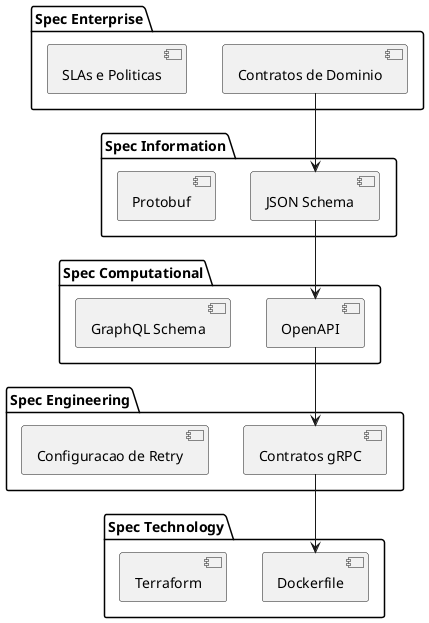
\includegraphics[width=0.85\textwidth]{imagens/01-modelagem-negocio-rm-odp-04-camadas-de-especificacao-baseadas-no-rm-odp.png}
    \caption{Camadas de Especificacao Baseadas no RM-ODP}
\end{figure}

\begin{description}[style=nextline]
    \item[Spec Enterprise] Contratos de domínio em linguagem natural estruturada
    --- ``O sistema deve processar pedidos em até 5 minutos após a confirmação
    do pagamento''. SLAs com valores numéricos. Políticas de compliance
    documentadas.

    \item[Spec Information] JSON Schema para validação de estruturas de dados.
    Protobuf para definição de mensagens entre serviços. Schemas de eventos
    para Domain Events.

    \item[Spec Computational] OpenAPI para APIs REST. GraphQL Schema para APIs
    GraphQL. AsyncAPI para interfaces assíncronas. Cada spec define contratos
    com tipos, validações e exemplos.

    \item[Spec Engineering] Contratos gRPC (\texttt{.proto} files). Configurações
    de retry, timeout e circuit breaker como código. Contratos de nível de
    serviço entre componentes.

    \item[Spec Technology] Dockerfiles para empacotamento. Terraform/Pulumi para
    infraestrutura. Helm charts para deploy em Kubernetes.
    \texttt{dependabot.yml} para gestão de dependências.
\end{description}

\subsection{Workflow SDD com RM-ODP}

O workflow completo de Spec Driven Development guiado pelo RM-ODP segue uma
progressão disciplinada:

\begin{enumerate}
    \item \textbf{Modelar o negócio com IDEF-0}: identificar funções, ICOMs e
    decomposição. Validar com stakeholders.

    \item \textbf{Definir Enterprise + Information Viewpoints}: documentar
    propósito, políticas, entidades, invariantes e ciclos de vida.

    \item \textbf{Especificar interfaces (Computational Viewpoint)}: criar
    OpenAPI specs, JSON Schemas, definições de eventos. Esses artefatos são
    revisáveis e testáveis antes de qualquer implementação.

    \item \textbf{Definir mecanismos (Engineering Viewpoint)}: especificar
    protocolos, estratégias de resiliência, padrões de consistência.

    \item \textbf{Gerar scaffolding a partir das specs}: usar ferramentas como
    \texttt{openapi-generator} para gerar código boilerplate a partir das specs
    OpenAPI, garantindo conformidade estrutural.

    \item \textbf{Implementar guiado pelas specs}: o código de implementação
    preenche o scaffolding, respeitando os contratos definidos.

    \item \textbf{Validar implementação contra as specs}: testes de contrato
    verificam que a implementação está conforme. Ferramentas como Pact, Dredd
    ou Schemathesis automatizam essa validação.

    \item \textbf{Evoluir specs e implementação em paralelo}: quando os
    requisitos mudam, a spec é atualizada \emph{primeiro}, depois a
    implementação segue.
\end{enumerate}

\textbf{Onde a IA entra nesse workflow}: LLMs podem gerar rascunhos de specs a
partir de descrições textuais, validar código contra specs existentes, sugerir
melhorias nas specs baseado em padrões do domínio, e gerar implementações a
partir de specs formais. O ponto crucial é que a spec funciona como
\textbf{âncora}: mesmo que a IA gere código imperfeito, a spec fornece
critérios objetivos para avaliar e corrigir.


% ============================================================
\section{RM-ODP com Assistentes de IA: Prompts Estruturados}
% ============================================================

Uma das aplicações mais imediatas e práticas do RM-ODP na era da IA é usá-lo
como \textbf{estrutura para prompts}. Um LLM que recebe contexto organizado
pelas cinco vistas produz resultados significativamente melhores do que um
que recebe uma descrição vaga do tipo ``crie um sistema de e-commerce''.

Vamos ver exemplos concretos de como cada vista pode ser usada para estruturar
prompts mais efetivos.

\subsection{Prompt para Modelagem de Domínio (Information Viewpoint)}

\begin{lstlisting}[language={}, caption={Prompt estruturado usando a Information Viewpoint}]
Voce e um arquiteto de software modelando o dominio
de um sistema de e-commerce multi-lojista.

CONTEXTO (Enterprise Viewpoint):
- Clientes compram de multiplos lojistas em um unico carrinho
- Pagamento unificado com split automatico para lojistas
- Entrega consolidada quando possivel
- Conformidade com LGPD e CDC

TAREFA (Information Viewpoint):
1. Identifique todas as entidades do dominio
2. Defina os relacionamentos entre elas (1:1, 1:N, N:M)
3. Liste as invariantes (regras que NUNCA podem ser violadas)
4. Modele o ciclo de vida de Pedido como maquina de estados
5. Identifique os Domain Events relevantes

RESTRICOES:
- Use DDD tatico (Entities, Value Objects, Aggregates)
- Cada Aggregate deve ter um unico Aggregate Root
- Priorize consistencia forte dentro do Aggregate
\end{lstlisting}

\subsection{Prompt para Geração de Specs (Computational Viewpoint)}

\begin{lstlisting}[language={}, caption={Prompt estruturado usando a Computational Viewpoint}]
Dado o seguinte modelo de dominio [cole o resultado anterior],
gere uma especificacao OpenAPI 3.1 para o PedidoService.

COMPUTATIONAL VIEWPOINT:
- Servico: PedidoService
- Responsabilidades: criar, cancelar, consultar pedidos
- Interacoes sincronas: EstoqueManager (reserva)
- Interacoes assincronas: publica PedidoCriado, PedidoCancelado

ENGINEERING VIEWPOINT (restricoes):
- Respostas devem incluir header X-Request-Id
- Erros seguem RFC 7807 (Problem Details)
- Paginacao via cursor (nao offset)
- Rate limit: 100 req/min por cliente

Gere a spec OpenAPI completa em YAML com:
- Schemas com exemplos e validacoes
- Respostas de erro para cada endpoint
- Descricoes em portugues brasileiro
\end{lstlisting}

Esses prompts estruturados produzem resultados vastamente superiores aos prompts
vagos porque fornecem ao LLM exatamente o que ele precisa: \textbf{contexto
delimitado} e \textbf{restrições claras}. O RM-ODP funciona como um template
mental que garante que nenhuma dimensão importante seja esquecida ao formular
o prompt.


% ============================================================
\section{TDD como Guardrail da IA}
% ============================================================

A inteligência artificial generativa pode produzir código funcional em segundos.
Mas ``funcional'' não significa ``correto'', e ``correto'' não significa ``bem
projetado''. Uma IA que recebe a instrução ``crie um serviço de pedidos'' vai
gerar algo que compila e talvez até rode --- mas que pode ignorar invariantes
do domínio, violar princípios de design, ou implementar uma lógica que é
\emph{plausível} mas não \emph{correta} para o seu contexto específico.

O Test-Driven Development (TDD) resolve esse problema ao inverter a equação:
em vez de pedir à IA para gerar código e depois verificar se está correto,
\textbf{você define o que é ``correto'' primeiro} (através de testes) e
então usa a IA para gerar uma implementação que satisfaça essa definição.

\begin{quote}
\textit{``Os testes definem o quê. A IA sugere o como. Você garante o design.''}
\end{quote}

\subsection{TDD + IA: O Workflow Detalhado}

O workflow de TDD com IA como implementadora segue um ciclo preciso:

\begin{figure}[htbp]
    \centering
    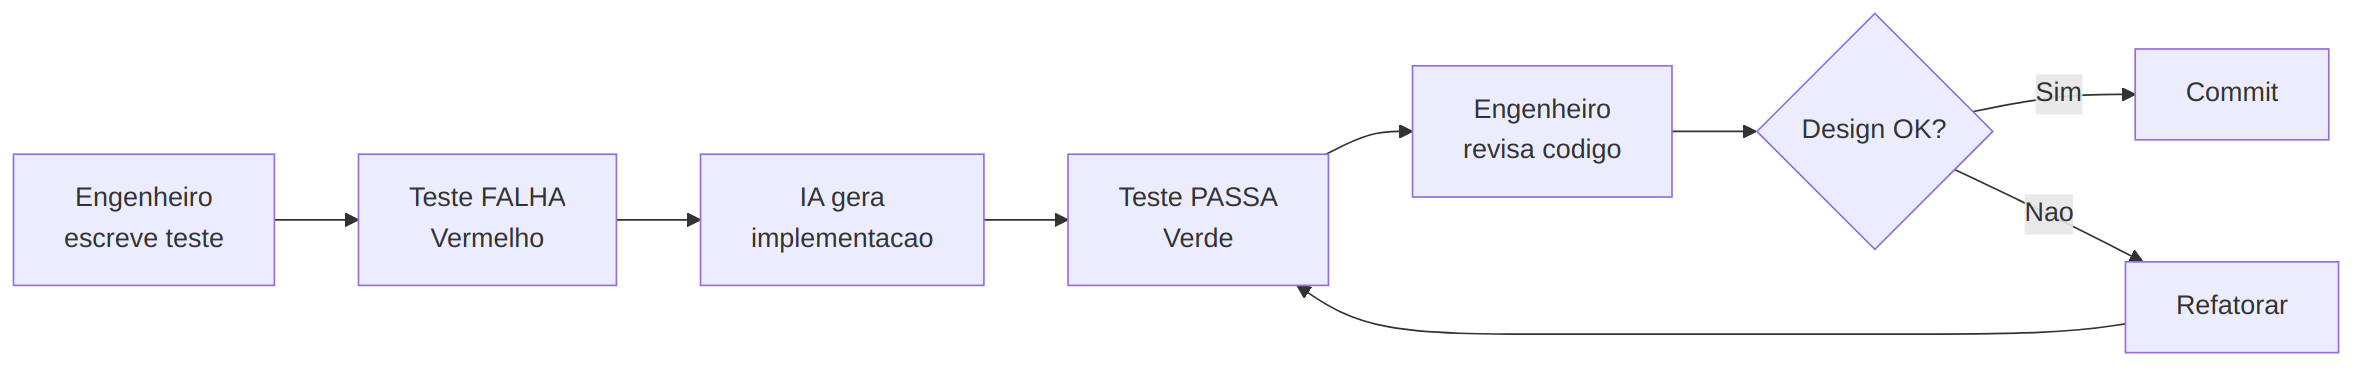
\includegraphics[width=0.85\textwidth]{imagens/01-modelagem-negocio-rm-odp-05-workflow-tdd-com-ia-como-implementadora.png}
    \caption{Workflow TDD com IA como Implementadora}
\end{figure}

\begin{enumerate}
    \item \textbf{O engenheiro escreve o teste} (vermelho). Esse teste é derivado
    diretamente das specs do RM-ODP: as invariantes da Information Viewpoint
    viram assertions, as pré-condições da Computational Viewpoint viram
    cenários de teste, os SLAs da Enterprise Viewpoint viram benchmarks.

    \item \textbf{A IA gera a implementação} para passar no teste (verde). O
    engenheiro fornece o teste junto com o contexto das vistas relevantes do
    RM-ODP, e a IA produz código que satisfaz os critérios definidos.

    \item \textbf{O engenheiro revisa o código gerado}. Aqui está o diferencial
    humano: a IA pode ter gerado código que passa no teste mas usa uma
    estrutura de dados ineficiente, viola o princípio de responsabilidade
    única, ou cria um acoplamento indesejado.

    \item \textbf{Refatoração colaborativa}: se o design não está adequado,
    o engenheiro refatora (possivelmente com auxílio da IA), sempre mantendo
    os testes verdes. Os testes são o \textbf{guardrail} que impede que a
    refatoração quebre o comportamento.
\end{enumerate}

\subsection{Exemplo Prático: Teste Derivado do RM-ODP}

Vamos escrever um teste que captura as invariantes da Information Viewpoint e os
contratos da Computational Viewpoint para a criação de pedidos:

\begin{lstlisting}[language=Python, caption={Testes derivados das vistas do RM-ODP}]
import pytest
from decimal import Decimal
from datetime import datetime


class TestCriarPedido:
    """Testes derivados da Computational Viewpoint.

    Cada teste mapeia para uma pre/pos-condicao ou
    invariante documentada no modelo RM-ODP.
    """

    async def test_cria_pedido_com_itens_validos(
        self, pedido_service, cliente_existente
    ):
        """Pos-condicao: pedido criado com status CRIADO."""
        request = CriarPedidoRequest(
            cliente_id=cliente_existente.id,
            itens=[
                ItemPedido(
                    sku="SKU-001",
                    quantidade=2,
                    preco_unitario=Decimal("49.90"),
                ),
            ],
        )

        pedido = await pedido_service.criar_pedido(request)

        assert pedido.status == StatusPedido.CRIADO
        assert pedido.valor_total == Decimal("99.80")
        assert pedido.cliente_id == cliente_existente.id
        assert len(pedido.itens) == 1

    async def test_rejeita_pedido_sem_itens(
        self, pedido_service, cliente_existente
    ):
        """Invariante: pedido deve ter ao menos um item."""
        with pytest.raises(ValueError):
            CriarPedidoRequest(
                cliente_id=cliente_existente.id,
                itens=[],
            )

    async def test_rejeita_quantidade_zero(
        self, pedido_service
    ):
        """Invariante: quantidade deve ser maior que zero."""
        with pytest.raises(ValueError):
            ItemPedido(
                sku="SKU-001",
                quantidade=0,
                preco_unitario=Decimal("49.90"),
            )

    async def test_reserva_estoque_ao_criar_pedido(
        self, pedido_service, estoque_manager_mock
    ):
        """Pos-condicao: estoque reservado apos criacao."""
        request = CriarPedidoRequest(
            cliente_id="cliente-123",
            itens=[
                ItemPedido(
                    sku="SKU-001",
                    quantidade=2,
                    preco_unitario=Decimal("49.90"),
                ),
            ],
        )

        await pedido_service.criar_pedido(request)

        estoque_manager_mock.reservar_itens.assert_called_once()

    async def test_publica_evento_pedido_criado(
        self, pedido_service, event_bus_mock
    ):
        """Pos-condicao: evento PedidoCriado publicado."""
        request = CriarPedidoRequest(
            cliente_id="cliente-123",
            itens=[
                ItemPedido(
                    sku="SKU-001",
                    quantidade=1,
                    preco_unitario=Decimal("29.90"),
                ),
            ],
        )

        await pedido_service.criar_pedido(request)

        event_bus_mock.publish.assert_called_once()
        evento = event_bus_mock.publish.call_args[0][0]
        assert evento.tipo == "PedidoCriado"
\end{lstlisting}

Observe como cada teste tem um comentário que rastreia sua origem para uma
invariante ou pós-condição documentada no modelo RM-ODP. Isso não é decoração
--- é \textbf{rastreabilidade}. Quando um teste falha, você sabe não apenas
\emph{o que} quebrou, mas \emph{qual requisito de negócio} está em risco.

\subsection{Guardrails em Múltiplos Níveis}

Os testes como guardrails operam em camadas progressivas, cada uma protegendo
um aspecto diferente do sistema:

\begin{description}[style=nextline]
    \item[Nível 1 --- Testes Unitários] Validam a lógica interna de cada
    componente isoladamente. Derivados das invariantes da Information Viewpoint
    e dos contratos da Computational Viewpoint. São rápidos (milissegundos) e
    devem cobrir todos os caminhos lógicos.

    \item[Nível 2 --- Testes de Contrato] Verificam que as interfaces entre
    componentes são respeitadas. Derivados da Computational e Engineering
    Viewpoints. Ferramentas como Pact garantem que consumidor e provedor
    concordam sobre o formato das mensagens.

    \item[Nível 3 --- Testes de Integração] Validam a interação real com
    bancos de dados, filas e APIs externas. Derivados da Engineering e
    Technology Viewpoints. Usam containers (Testcontainers) para simular
    a infraestrutura real.

    \item[Nível 4 --- Testes End-to-End] Validam fluxos completos de negócio
    do ponto de vista do usuário. Derivados da Enterprise Viewpoint. São os
    mais lentos e frágeis, mas os que mais se aproximam da experiência real.
\end{description}

A IA navega \textbf{dentro} dos guardrails definidos por esses testes.
O engenheiro define \textbf{onde} os guardrails estão. Essa divisão de
responsabilidades é a chave para usar IA generativa de forma produtiva
e segura no desenvolvimento de software --- tema que exploraremos com
muito mais profundidade no Capítulo~4.


% ============================================================
\section{Conclusão}
% ============================================================

Ao longo deste capítulo, percorremos um caminho que vai da compreensão do
negócio até a validação do código, usando IDEF-0 e RM-ODP como guias
estruturantes. Esses frameworks não são burocracia --- são \textbf{disciplina
de pensamento}. Eles forçam o engenheiro a responder perguntas que, se
ignoradas, inevitavelmente se transformam em bugs, retrabalho e frustração.

O IDEF-0 nos ensina a decompor processos de negócio de forma rigorosa,
garantindo que entendemos o problema antes de propor soluções. O RM-ODP nos
oferece cinco lentes complementares para examinar o sistema sob todos os
ângulos relevantes, da motivação empresarial às escolhas tecnológicas. Juntos,
eles criam uma cadeia de rastreabilidade que conecta cada linha de código a
um propósito de negócio.

O Spec Driven Development transforma os modelos conceituais em especificações
formais e executáveis --- artefatos que não apenas documentam a intenção, mas
a \emph{validam} automaticamente. E o TDD, especialmente quando combinado com
IA generativa, cria os guardrails que garantem que o código gerado serve ao
propósito definido nas especificações.

Na era dos LLMs, esses conceitos ganham uma dimensão adicional. A IA pode
gerar código em velocidade sobre-humana, mas sem contexto estruturado, ela
gera o código \emph{errado} rapidamente. IDEF-0 e RM-ODP fornecem esse
contexto. As specs fornecem os critérios de validação. Os testes fornecem
os guardrails. O engenheiro orquestra tudo isso, exercendo o que chamamos no
Capítulo~0 de \textbf{pensamento de engenharia} --- a capacidade de pensar
sistematicamente sobre problemas complexos antes de resolvê-los.

No próximo capítulo, aprofundaremos a conversa sobre arquitetura de software,
explorando como tomar decisões arquiteturais informadas \emph{antes} de
escrever código --- e como documentar essas decisões de forma que sobrevivam
ao tempo e à rotatividade de equipe.


% ============================================================
\section*{Exercícios}
% ============================================================

\begin{enumerate}
    \item \textbf{Modelagem IDEF-0 --- Sistema Universitário.}
    Modele com IDEF-0 o processo de matrícula em uma universidade. Comece pelo
    diagrama A-0 (contexto) e decomponha em pelo menos dois níveis. Para cada
    nível, identifique explicitamente todos os elementos ICOM (Inputs, Controls,
    Outputs, Mechanisms). Dica: os Controls incluem o regimento acadêmico, os
    pré-requisitos das disciplinas e o calendário letivo.

    \item \textbf{Cinco Vistas do RM-ODP.}
    Para o mesmo sistema de matrícula universitária, elabore as cinco vistas do
    RM-ODP. Na Enterprise Viewpoint, identifique pelo menos 5 stakeholders com
    interesses distintos. Na Information Viewpoint, modele as entidades Aluno,
    Disciplina, Turma e Matrícula com suas invariantes. Na Computational
    Viewpoint, defina pelo menos 3 componentes com suas interfaces. Compare
    o resultado com uma descrição informal que você faria sem o framework.
    O que o framework revelou que a descrição informal escondeu?

    \item \textbf{Spec OpenAPI a partir da Computational Viewpoint.}
    Escolha um dos componentes definidos no exercício anterior e escreva uma
    especificação OpenAPI 3.0 completa para ele, incluindo: schemas com
    validações, endpoints com descrições, respostas de sucesso e de erro,
    e pelo menos um exemplo por endpoint. Em seguida, use uma ferramenta
    de geração de código (como \texttt{openapi-generator}) para gerar o
    scaffolding e implemente a lógica de negócio.

    \item \textbf{TDD com IA.}
    Escolha uma das invariantes da Information Viewpoint do exercício 2 e
    escreva um teste automatizado (em Python com pytest ou em TypeScript
    com Jest) que valide essa invariante. Execute o teste (ele deve falhar
    --- vermelho). Em seguida, peça a um LLM para gerar a implementação
    que faça o teste passar. Revise o código gerado: ele respeita os
    princípios de design que estudamos? Compare a qualidade do código
    gerado com TDD versus código gerado sem testes prévios.

    \item \textbf{Matriz de Rastreabilidade.}
    Crie uma matriz de rastreabilidade completa para um projeto real ou
    fictício, mapeando cada elemento IDEF-0 para as cinco vistas do
    RM-ODP (use a Tabela~\ref{tab:idef-odp-mapping} como referência).
    Identifique pelo menos 3 lacunas (gaps) na matriz --- elementos que
    existem em uma vista mas não têm correspondência em outra. Para cada
    lacuna, proponha uma ação corretiva.

    \item \textbf{Prompt Engineering com RM-ODP.}
    Escolha um domínio de negócio que você conheça bem (pode ser o da sua
    empresa ou um domínio de interesse pessoal). Escreva 3 prompts
    estruturados usando o RM-ODP como template: um para modelagem de
    domínio (Information Viewpoint), um para geração de spec OpenAPI
    (Computational Viewpoint) e um para definição de infraestrutura
    (Technology Viewpoint). Execute os prompts em um LLM e avalie
    criticamente os resultados. O que o LLM acertou? O que ele inventou?
    O que ele deixou de fora?
\end{enumerate}
